\chapter{Realization}

In the following chapter, we describe the realization of the software system. In section \ref{sec:structure}, we give an overview of the different components and how they interact with each other. In section \ref{sec:changes}, we list the changes which have to be made to existing components.

\section{Structure}\label{sec:structure}

The system consists of three major components: the \emph{Bot Service}, the \emph{Mensa Service} and the \emph{MobSOS CCA} backend service.

The MobSOS CCA backend service has access to three different databases. First, the MobSOS CCA service can access the food reviews, which are stored inside the las2peer database of the Mensa Service. Second, the system can access \emph{Mediabase} data, which contains data from reviews, made outside of the las2peer system. This data will be collected by a crawler bot, which searches Google and Twitter for reviews of the canteen. Those two databases provide the information quality factors of the MobSOS success model.
Third, the CCA service can also access monitoring data generated by the Bot and the Mensa Service. Those monitoring messages provide the system quality factors of the MobSOS success model.

The Bot Service acts as an interface between the user, and the backend services Mensa Service and CCA service.
The Bot Service communicates with the \emph{Mensa Service} in order to get the menu for the canteen. Additionally, the bot can send requests to the Mensa service, telling it to add, or modify, reviews. The reviews are stored inside a las2peer database.
The Bot Service communicates with the CCA system in order to retrieve data of the success model. Furthermore, the MobSOS CCA system can also be used to modify the success model of the system. The bot contains a service, which provides the visualisations for given success data as a picture which can be sent to the user in chat.

\section{Changes to Core Components} \label{sec:changes}

The Social Bot Framework needs to be extended, such that the bot is able to listen to specific mentions in group chats and filtering out the rest of the conversations, such that the bot can be integrated in group chats, as a quiet agent.

\begin{figure}[h]
    \centering
    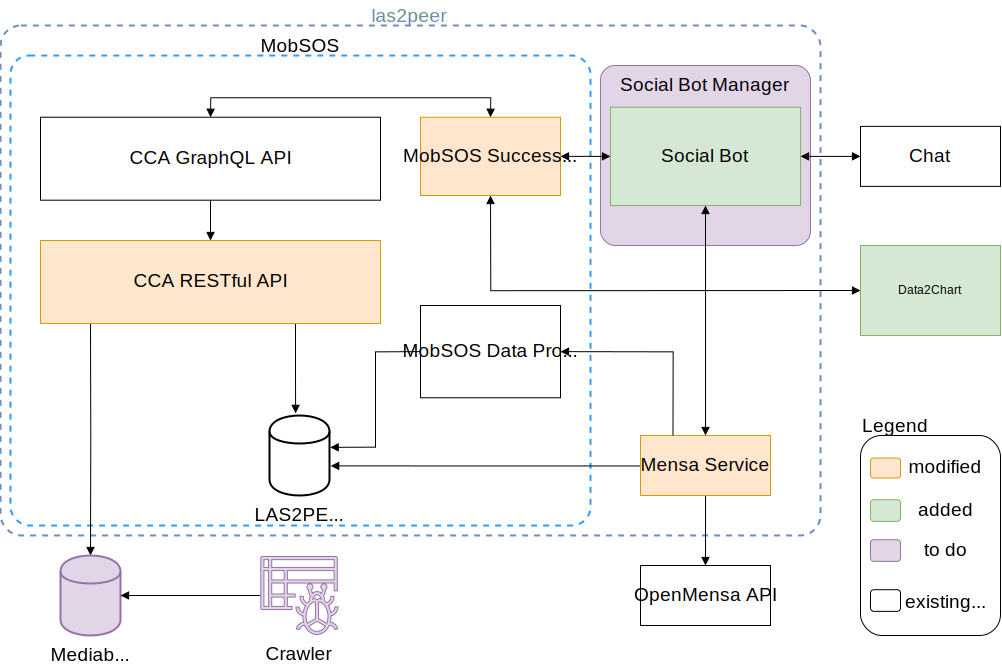
\includegraphics[width=\linewidth]{realization/components_overview.png}
    \caption{Overview of the different components}
    \label{fig:componentsOverview}
\end{figure}

\begin{figure}[h]
    \centering
    \includegraphics[width=\linewidth]{realization/chat_mockup.png}
    \caption{Example use of community Service with the Bot}
    \label{fig:chatMockup}
\end{figure}

\begin{figure}[h]
    \centering
    \includegraphics[width=0.5\linewidth]{realization/visual_req.png}
    \caption{Example of a chat interaction with the Bot}
    \label{fig:visualReq}
\end{figure}